\chapter{The Outlier Anchor Node Placements}
As seen in the previous chapter, there are some anchor node placements that are significantly worse than the average case.   In this chapter, we explore in more detail the cause of these outliers and more importantly, is this condition detectable in the real world.

\section{The Cause}
Figure~\ref{fig:outlier1} shows a network difference plot of an example outlier anchor node placement for a random network. A line is drawn between the real location and the calculated location.  For comparison, Figure~\ref{fig:normal1} is a randomly chosen normal case. This representation gives a clear indication that the reflection component of the final linear transformation is to blame for the extremely poor results.  

\begin{figure}
  \centering
	\subfloat[An outlier network difference]{\label{fig:outlier1}
		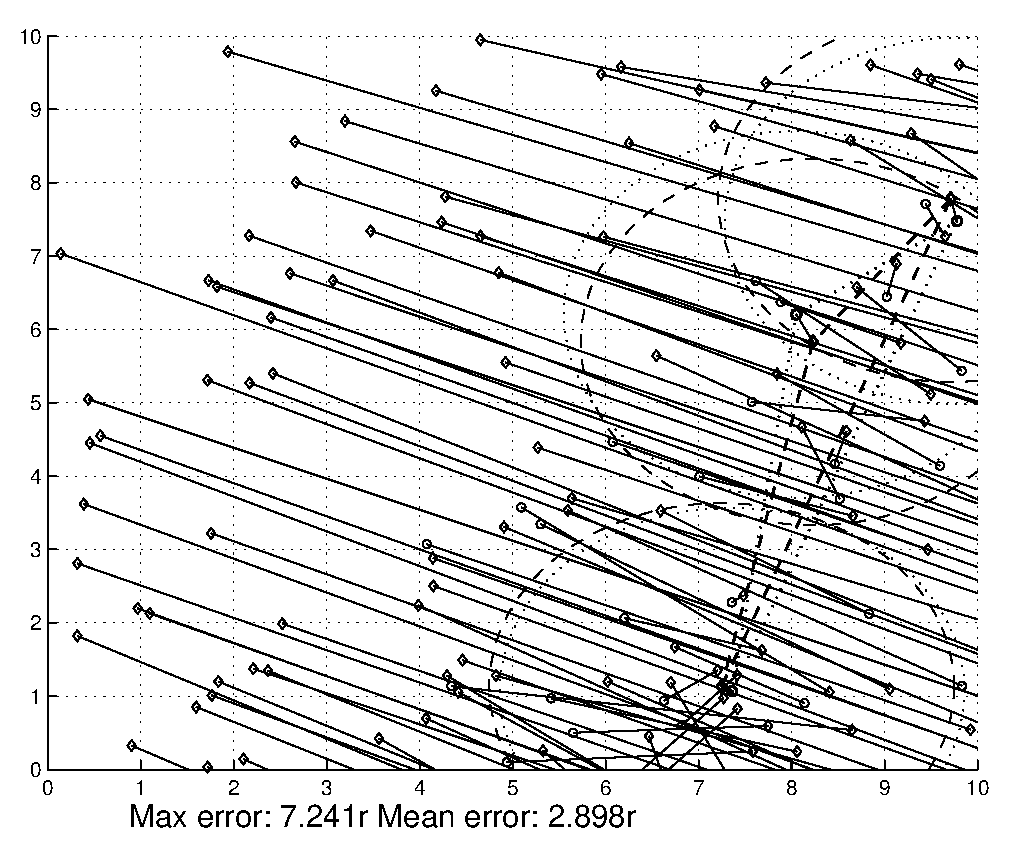
\includegraphics[width=0.5\textwidth]{outliers/AS6/AS6NetworkDiff9}}
	\subfloat[A normal network difference]{\label{fig:normal1}
		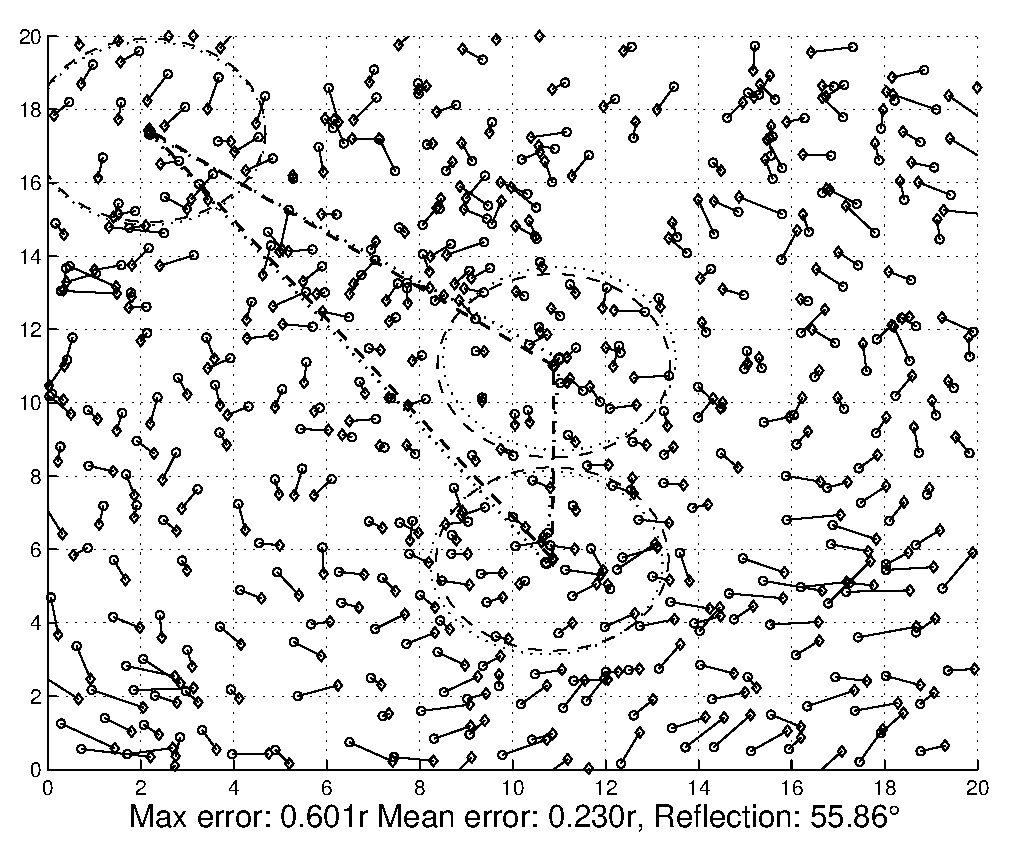
\includegraphics[width=0.5\textwidth]{outliers/normal1}}		
	\label{fig:outliernetworkdiff}
	\caption{}
\end{figure}

\section{Avoiding the Outlier}

Unfortunately, simply disabling the reflection component of the Procrustes transformation algorithm does not solve the problem.  The output of the Procrustes algorithm is a linear transformation which includes a rotation or reflection matrix.  If the determinant of that matrix is +1, then the resulting transformation has rotation, with an angle as in Equation~\ref{eqn:rotmatrix}.  

\begin{equation}
	\det{(T)}=+1 \Rightarrow ~Rotation ~with ~T=
	\begin{bmatrix}
	\cos{\theta} & -\sin{\theta} \\ 
	\sin{\theta} & \cos{\theta}\end{bmatrix}
	\label{eqn:rotmatrix} 
\end{equation}

If the determinant is -1, then the resulting transformation has reflection component, across a line at angle as shown in Equation~\ref{eqn:refmatrix}. 

\begin{equation}
	\det{(T)}=-1 \Rightarrow ~Reflection ~with ~T=
	\begin{bmatrix}
	\cos{2{\theta}} & \sin{2{\theta}} \\ 
	\sin{2{\theta}} & -\cos{2{\theta}}\end{bmatrix}
	\label{eqn:refmatrix} 
\end{equation}

Figure~\ref{fig:rotref} shows the rotation and reflection distributions of two different networks, for a random of set of anchor sets for each network.  In both networks, and with consistency across others, the bulk of the data points have the same angle of either rotation or reflection, while the outliers have the opposite property with a wide variance in the angle.  However, between networks, it is not consistently wither rotation or reflection.  Therefore, relying on the determinant of the transformation is not a sufficient indicator of a network planner knowing that an outlier case has been hit and thus the localization results are essentially useless.

\begin{figure}
  \centering
	\subfloat[]{\label{fig:rotref1}
		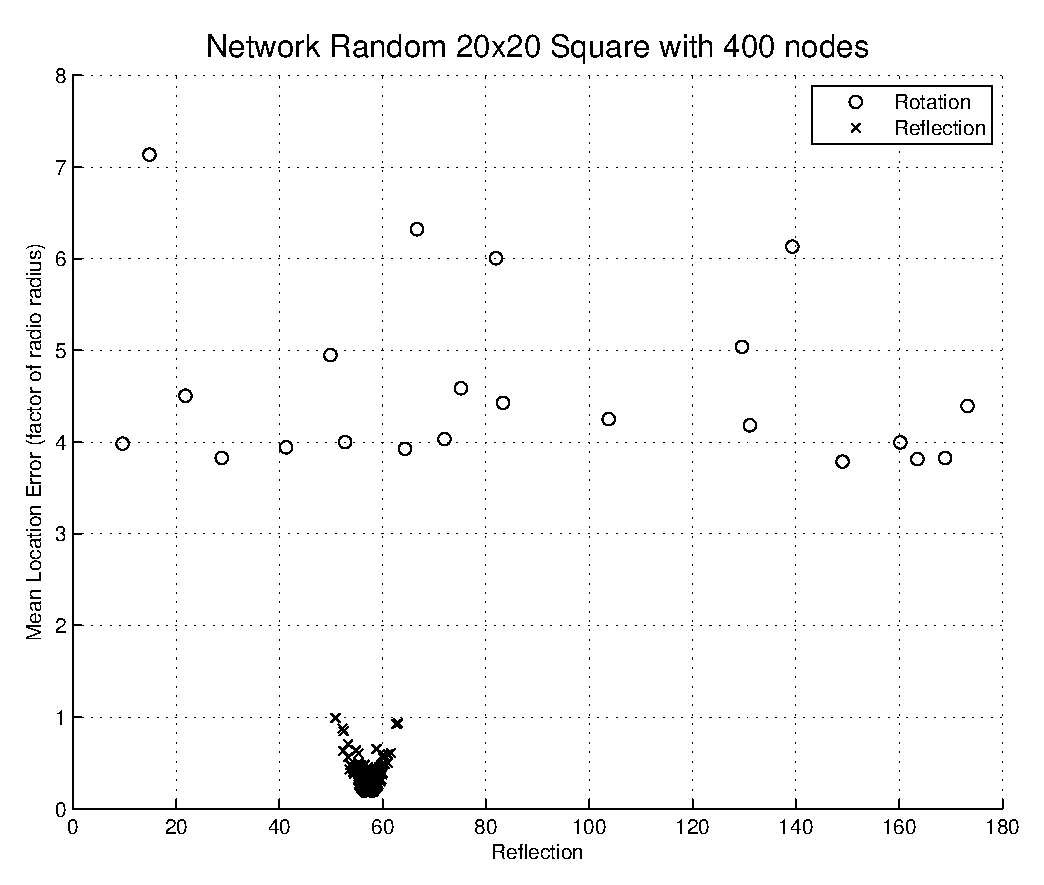
\includegraphics[width=0.5\textwidth]{rotref1}}
	\subfloat[]{\label{fig:rotref2}
		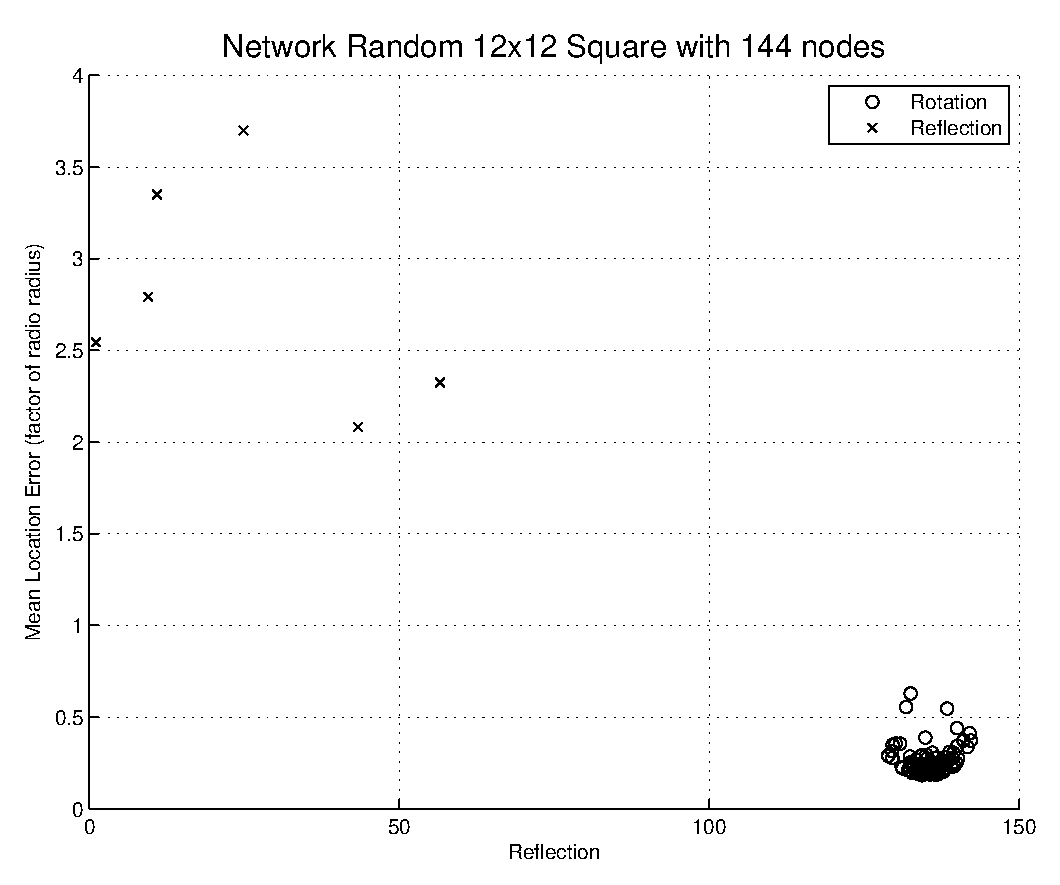
\includegraphics[width=0.5\textwidth]{rotref2}}		
	\caption{Rotation and Reflection versus Mean Location Error}	
	\label{fig:rotref}
\end{figure}

Further, the Procrustes algorithm itself provides a measure of the dissimilarity.  Specifically, it is the minimized value of sum of squared errors\cite{procrustes-matlab}.  As shown in Figure~\ref{fig:dissimilarity}, it is not a good indicator of the transformation as it pertains to the entire network.  This is because the Procrustes algorithm is only performed on the anchor nodes themselves and for those nodes themselves, the transformation is good.

\begin{figure}
  \centering
	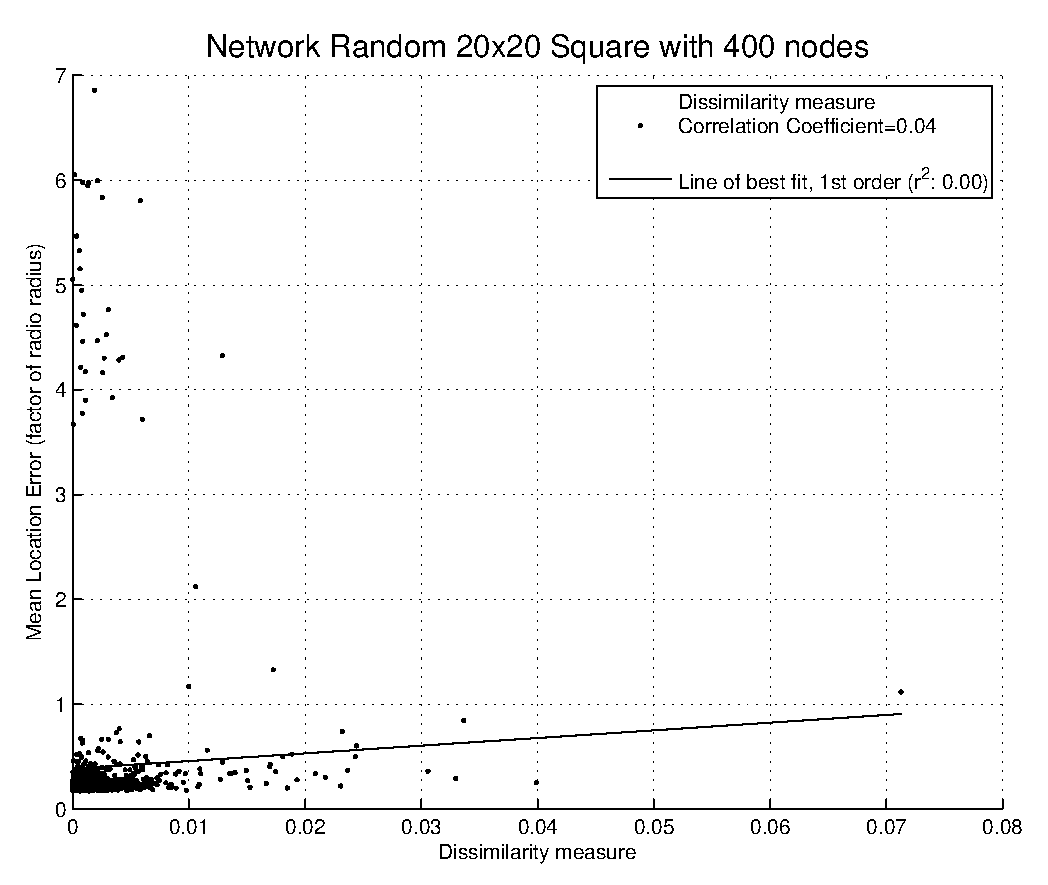
\includegraphics[width=0.5\textwidth]{dissimilarity}
	\caption{Procrustes dissimilarity measure}	
	\label{fig:dissimilarity}
\end{figure}

As shown in Figure~\ref{fig:rotref}, each network has a \emph{natural} rotation or reflection angle to provide accurate localization.  As the linear transformation moves away from that angle, the errors increase.  Unfortunately, there is no direct indicator that a particular anchor set generates a transformation with an incorrect angle.  Therefore, network planners must avoid all anchor sets that could potentially generate such an angle.  As shown in the Section~\ref{sec:anchorTriangle}, the area and height of the triangle formed by the anchor nodes are a good indicator of the possibility of a poor transformation angle.  But how flat of a triangle is too flat?

\section{Minimum Area and Height of the Anchor Triangle} 
